\documentclass[12pt,a4paper]{article}
\usepackage{longtable}
\usepackage[LGR,T1]{fontenc}
\usepackage{lscape}
%\usepackage{pdfsync}
\usepackage[shortlabels]{enumitem}
\usepackage{multirow}
\usepackage{fancyhdr}
\usepackage{graphicx}
\usepackage{lastpage}
\usepackage{afterpage}
\usepackage{lettrine}
\usepackage{color,soul}
\usepackage[svgnames]{xcolor}
\usepackage{colortbl}
\usepackage{enumitem}
\usepackage{tikz}
\usepackage{titlesec}
\usepackage{eurosym}
\usepackage{amsmath}
\usepackage{subcaption}

%Palatino font
%\usepackage{pxfonts}
%\usepackage{libertine}
\usepackage[scaled=0.88]{beraserif}
\usepackage[scaled=0.85]{berasans}
\usepackage[scaled=0.84]{beramono}
\usepackage{mathpazo}
%\linespread{1.05}
\usepackage[T1,small,euler-digits]{eulervm}

\usepackage[citestyle=apa,style=apa,backend=biber,url=false,uniquename=false, useprefix=true, doi=false]{biblatex}
% \renewcommand*{\nameyeardelim}{\addcomma\space} % https://tex.stackexchange.com/questions/134063/how-to-add-a-comma-between-author-and-year
\usepackage{dsfont} % for fancy R
\AtEveryBibitem{%
  \clearfield{note}%
}
% \renewcommand*{\nameyeardelim}{\addcomma\space} % https://tex.stackexchange.com/questions/134063/how-to-add-a-comma-between-author-and-year
\usepackage{dsfont} % for fancy R
\AtEveryBibitem{%
  \clearfield{note}%
}
\setcounter{biburlnumpenalty}{100} % https://tex.stackexchange.com/questions/50957/handling-overflows-in-biblatex-bibliographies
\addbibresource{biblio.bib} % Imports bibliography file

\usepackage[nomessages]{fp}


 \definecolor{bleuUCLclair}{rgb}{.09, 0.569, 1}
\definecolor{bleuUCLfonce}{rgb}{ .13, .52, .86}
\definecolor{redBurn}{rgb}{.91, 0.29, 0.08}

\usepackage[colorlinks=true,urlcolor=LightSeaGreen,linkcolor=black]{hyperref}
\addtolength{\topmargin}{-1.5cm}
\addtolength{\textheight}{1.5cm}
\addtolength{\textwidth}{2cm}
\addtolength{\footskip}{2cm}
\setlength{\evensidemargin}{-0.5cm}
\setlength{\oddsidemargin}{-0.5cm}
\setlength{\arrayrulewidth}{0.25pt}

\renewcommand{\baselinestretch}{1.1} % Interligne


\newenvironment{maliste}%
{ \begin{list}%
    {\textcolor{bleuUCLfonce}{$\bullet$}\hspace{0.5cm}}%
    {\setlength{\labelwidth}{50pt}%
     \setlength{\leftmargin}{25pt}%
     \setlength{\itemsep}{30pt}}}%
{ \end{list} }

%\renewcommand{\headrulewidth}{0.0pt}
%\newcommand{\clearemptydoublepage}{%
%   \newpage{\pagestyle{empty}\cleardoublepage}}




%section like title in longtable
\newcommand{\seclong}[1]{\multicolumn{2}{@{}l}{{\Large\sffamily #1}} 
\vspace{0.5cm}
\\}

%enumerate on two columns
\newcounter{listlong}
\newcommand{\newlistlong}{\setcounter{listlong}{1}}
\newcommand{\iteml}[1]{%
\hspace{4.5cm}\textcolor{redBurn}{\arabic{listlong}}\stepcounter{listlong}%
&%
#1%
 
\\%
}

%left in column
\newcommand{\lcol}[1]{%
\begin{minipage}[t]{.35\textwidth}%

#1%

\end{minipage}%
}

\title{\vspace{-1cm}
\begin{flushleft} {\sffamily Revisions to \emph{``On the estimation of the number of components in multivariate functional principal component analysis''}}\end{flushleft}}
\date{\vspace{-1.7cm}\begin{flushleft}\sffamily Steven Golovkine,
Edward Gunning,
Andrew J. Simpkin,
and 
Norma Bargary.
\end{flushleft}}


\pagestyle{fancy} 
\fancyhf{}
\fancyfoot[R]{\sffamily\thepage\ / \pageref{LastPage}}
  \fancyfoot[L]{ }

\fancypagestyle{plain}{%
  \fancyhf{}%
  \fancyfoot[R]{\sffamily\thepage\ / \pageref{LastPage}}
  \fancyfoot[L]{ }
}

\renewcommand{\headrulewidth}{0.0pt}


\newcommand{\hlc}[2][yellow]{ {\sethlcolor{#1} \hl{$^{TODO:}$#2}} }

\newcommand{\paolo}[2][green]{ {\sethlcolor{#1} \hl{$^{P:}$#2}} }


\titleformat{\section}
{\bfseries\scshape}{Reviewer \# \thesection}{1em}{}

\titleformat{\subsection}
{\normalfont\scshape}{Comment \# \thesubsection}{1em}{}

\usepackage[framemethod=default]{mdframed}
%\mdfsetup{skipabove=\topskip,skipbelow=\topskip}

\global\mdfdefinestyle{comments}{%
     linecolor=FireBrick!50,linewidth=0.1cm,backgroundcolor=FireBrick!5,%
     leftmargin=-0.5cm,rightmargin=-0.5cm, innerleftmargin=0.4cm,innerrightmargin=0.4cm,
     topline=false,bottomline=false
}

\global\mdfdefinestyle{changes}{%
     linecolor=DarkSeaGreen!10,linewidth=0.05cm,backgroundcolor=DarkSeaGreen!10,%
     leftmargin=-0.1cm,rightmargin=-0.1cm, innerleftmargin=0.1cm,innerrightmargin=0.1cm,
          topline=false,bottomline=false
}

\global\mdfdefinestyle{replies}{%
    linecolor=DodgerBlue!10,linewidth=0.05cm,backgroundcolor=DodgerBlue!1,%
    leftmargin=-0.1cm,rightmargin=-0.1cm, innerleftmargin=0.1cm,innerrightmargin=0.1cm,
    rightline=false,leftline=false
}
  
  \renewcommand{\subsectionautorefname}{Comment}
  
\newcommand{\comments}[1]{\subsection{}
\begin{mdframed}[style=comments] 
        \textit{#1}
\end{mdframed}}



\newcommand{\reply}[1]{
    \noindent\textbf{Reply:}

\begin{mdframed}[style=replies] 
    #1
\end{mdframed}
}

\newcommand{\changes}[1]{
    \noindent\textbf{Changes:}
    \vspace{-5pt}
\begin{mdframed}[style=changes] 
    #1
\end{mdframed}}

%DIF PREAMBLE EXTENSION ADDED BY LATEXDIFF
%DIF UNDERLINE PREAMBLE %DIF PREAMBLE
\RequirePackage[normalem]{ulem} %DIF PREAMBLE
\RequirePackage{color}\definecolor{RED}{rgb}{1,0,0}\definecolor{BLUE}{rgb}{0,0,1} %DIF PREAMBLE
\providecommand{\DIFaddtex}[1]{{\protect\color{blue}\uwave{#1}}} %DIF PREAMBLE
\providecommand{\DIFdeltex}[1]{{\protect\color{red}\sout{#1}}}                      %DIF PREAMBLE
%DIF SAFE PREAMBLE %DIF PREAMBLE
\providecommand{\DIFaddbegin}{} %DIF PREAMBLE
\providecommand{\DIFaddend}{} %DIF PREAMBLE
\providecommand{\DIFdelbegin}{} %DIF PREAMBLE
\providecommand{\DIFdelend}{} %DIF PREAMBLE
\providecommand{\DIFmodbegin}{} %DIF PREAMBLE
\providecommand{\DIFmodend}{} %DIF PREAMBLE
%DIF FLOATSAFE PREAMBLE %DIF PREAMBLE
\providecommand{\DIFaddFL}[1]{\DIFadd{#1}} %DIF PREAMBLE
\providecommand{\DIFdelFL}[1]{\DIFdel{#1}} %DIF PREAMBLE
\providecommand{\DIFaddbeginFL}{} %DIF PREAMBLE
\providecommand{\DIFaddendFL}{} %DIF PREAMBLE
\providecommand{\DIFdelbeginFL}{} %DIF PREAMBLE
\providecommand{\DIFdelendFL}{} %DIF PREAMBLE
%DIF HYPERREF PREAMBLE %DIF PREAMBLE
\providecommand{\DIFadd}[1]{\texorpdfstring{\DIFaddtex{#1}}{#1}} %DIF PREAMBLE
\providecommand{\DIFdel}[1]{\texorpdfstring{\DIFdeltex{#1}}{}} %DIF PREAMBLE
\newcommand{\DIFscaledelfig}{0.5}
%DIF HIGHLIGHTGRAPHICS PREAMBLE %DIF PREAMBLE
\RequirePackage{settobox} %DIF PREAMBLE
\RequirePackage{letltxmacro} %DIF PREAMBLE
\newsavebox{\DIFdelgraphicsbox} %DIF PREAMBLE
\newlength{\DIFdelgraphicswidth} %DIF PREAMBLE
\newlength{\DIFdelgraphicsheight} %DIF PREAMBLE
% store original definition of \includegraphics %DIF PREAMBLE
\LetLtxMacro{\DIFOincludegraphics}{\includegraphics} %DIF PREAMBLE
\newcommand{\DIFaddincludegraphics}[2][]{{\color{blue}\fbox{\DIFOincludegraphics[#1]{#2}}}} %DIF PREAMBLE
\newcommand{\DIFdelincludegraphics}[2][]{% %DIF PREAMBLE
    \sbox{\DIFdelgraphicsbox}{\DIFOincludegraphics[#1]{#2}}% %DIF PREAMBLE
    \settoboxwidth{\DIFdelgraphicswidth}{\DIFdelgraphicsbox} %DIF PREAMBLE
    \settoboxtotalheight{\DIFdelgraphicsheight}{\DIFdelgraphicsbox} %DIF PREAMBLE
    \scalebox{\DIFscaledelfig}{% %DIF PREAMBLE
        \parbox[b]{\DIFdelgraphicswidth}{\usebox{\DIFdelgraphicsbox}\\[-\baselineskip] \rule{\DIFdelgraphicswidth}{0em}}\llap{\resizebox{\DIFdelgraphicswidth}{\DIFdelgraphicsheight}{% %DIF PREAMBLE
                \setlength{\unitlength}{\DIFdelgraphicswidth}% %DIF PREAMBLE
                \begin{picture}(1,1)% %DIF PREAMBLE
                    \thicklines\linethickness{2pt} %DIF PREAMBLE
                    {\color[rgb]{1,0,0}\put(0,0){\framebox(1,1){}}}% %DIF PREAMBLE
                    {\color[rgb]{1,0,0}\put(0,0){\line( 1,1){1}}}% %DIF PREAMBLE
                    {\color[rgb]{1,0,0}\put(0,1){\line(1,-1){1}}}% %DIF PREAMBLE
                \end{picture}% %DIF PREAMBLE
            }\hspace*{3pt}}} %DIF PREAMBLE
} %DIF PREAMBLE
\LetLtxMacro{\DIFOaddbegin}{\DIFaddbegin} %DIF PREAMBLE
\LetLtxMacro{\DIFOaddend}{\DIFaddend} %DIF PREAMBLE
\LetLtxMacro{\DIFOdelbegin}{\DIFdelbegin} %DIF PREAMBLE
\LetLtxMacro{\DIFOdelend}{\DIFdelend} %DIF PREAMBLE
\DeclareRobustCommand{\DIFaddbegin}{\DIFOaddbegin \let\includegraphics\DIFaddincludegraphics} %DIF PREAMBLE
\DeclareRobustCommand{\DIFaddend}{\DIFOaddend \let\includegraphics\DIFOincludegraphics} %DIF PREAMBLE
\DeclareRobustCommand{\DIFdelbegin}{\DIFOdelbegin \let\includegraphics\DIFdelincludegraphics} %DIF PREAMBLE
\DeclareRobustCommand{\DIFdelend}{\DIFOaddend \let\includegraphics\DIFOincludegraphics} %DIF PREAMBLE
\LetLtxMacro{\DIFOaddbeginFL}{\DIFaddbeginFL} %DIF PREAMBLE
\LetLtxMacro{\DIFOaddendFL}{\DIFaddendFL} %DIF PREAMBLE
\LetLtxMacro{\DIFOdelbeginFL}{\DIFdelbeginFL} %DIF PREAMBLE
\LetLtxMacro{\DIFOdelendFL}{\DIFdelendFL} %DIF PREAMBLE
\DeclareRobustCommand{\DIFaddbeginFL}{\DIFOaddbeginFL \let\includegraphics\DIFaddincludegraphics} %DIF PREAMBLE
\DeclareRobustCommand{\DIFaddendFL}{\DIFOaddendFL \let\includegraphics\DIFOincludegraphics} %DIF PREAMBLE
\DeclareRobustCommand{\DIFdelbeginFL}{\DIFOdelbeginFL \let\includegraphics\DIFdelincludegraphics} %DIF PREAMBLE
\DeclareRobustCommand{\DIFdelendFL}{\DIFOaddendFL \let\includegraphics\DIFOincludegraphics} %DIF PREAMBLE
%DIF LISTINGS PREAMBLE %DIF PREAMBLE
\RequirePackage{listings} %DIF PREAMBLE
\RequirePackage{color} %DIF PREAMBLE
\lstdefinelanguage{DIFcode}{ %DIF PREAMBLE
    %DIF DIFCODE_UNDERLINE %DIF PREAMBLE
    moredelim=[il][\color{red}\sout]{\%DIF\ <\ }, %DIF PREAMBLE
    moredelim=[il][\color{blue}\uwave]{\%DIF\ >\ } %DIF PREAMBLE
} %DIF PREAMBLE
\lstdefinestyle{DIFverbatimstyle}{ %DIF PREAMBLE
    language=DIFcode, %DIF PREAMBLE
    basicstyle=\ttfamily, %DIF PREAMBLE
    columns=fullflexible, %DIF PREAMBLE
    keepspaces=true %DIF PREAMBLE
} %DIF PREAMBLE
\lstnewenvironment{DIFverbatim}{\lstset{style=DIFverbatimstyle}}{} %DIF PREAMBLE
\lstnewenvironment{DIFverbatim*}{\lstset{style=DIFverbatimstyle,showspaces=true}}{} %DIF PREAMBLE
%DIF END PREAMBLE EXTENSION ADDED BY LATEXDIFF



\begin{document}


\qquad

\qquad

\qquad


\qquad

\qquad

\qquad

\newcommand{\thedate}{\today}

\thedate

\qquad

\qquad

\qquad



Dear Editor,

\qquad


We would be very grateful if you would consider this revision, entitled \emph{`On the estimation of the number of components in multivariate functional principal component analysis'} for publication in \emph{Communications in Statistics - Simulation and Computation}. We were able to address the comments made by the reviewers and to strengthen our results. A point-to-point reply is provided below. 

\quad

We quite naturally hope that this version matches reviewers' expectations, and we thank you in advance for your consideration.



\quad


Sincerely, 

\medskip



 Steven Golovkine 
 \\(on behalf of the co-authors  Edward Gunning, Andrew J. Simpkin and Norma Bargary)





\newpage

\maketitle

\noindent The changes are in \textcolor{blue}{blue} in the main text.
\vspace*{1cm}

\section{}

\comments{Although I understand how $s_1, \dots , s_p$ are obtained, the authors need to provide a more detailed explanation of how these values are generated using a Bernoulli distribution, for example.}

\reply{We have added the sentence ``generated according to a Bernoulli distribution'' to the text to clarify how these values are obtained.}


\comments{It would be helpful to simulate a case with irregular time points, where each function has different time points. Moreover, the time points for each function do not need to be regular. I recommend that the authors consider these situations.}

\reply{Thank you for your suggestion to include a case with irregular functional data. We did the analysis with sparse data. The sparsification consisted in randomly removing between $40\%$ and $60\%$ of the $S$ sampling points for each curve. Figure~\ref{fig:ncomp} presents the results of the estimation the eigenvalues. The case where $S = 25$ is not included because the number of points (after sparsification) is not enough to consistently estimated $10$ univariate components for each univariate feature. The results are similar to the dense case (when all the sampling points are observed). The estimation of the last multivariate eigencomponents is not good. We choose to not include the graph in the paper to not overload it. We prefer to keep the message of the paper simple: even in simple situation (such as dense functional data), be careful when choosing the number of multivariate components to retain.}
\begin{figure}[!h]
     \centering
    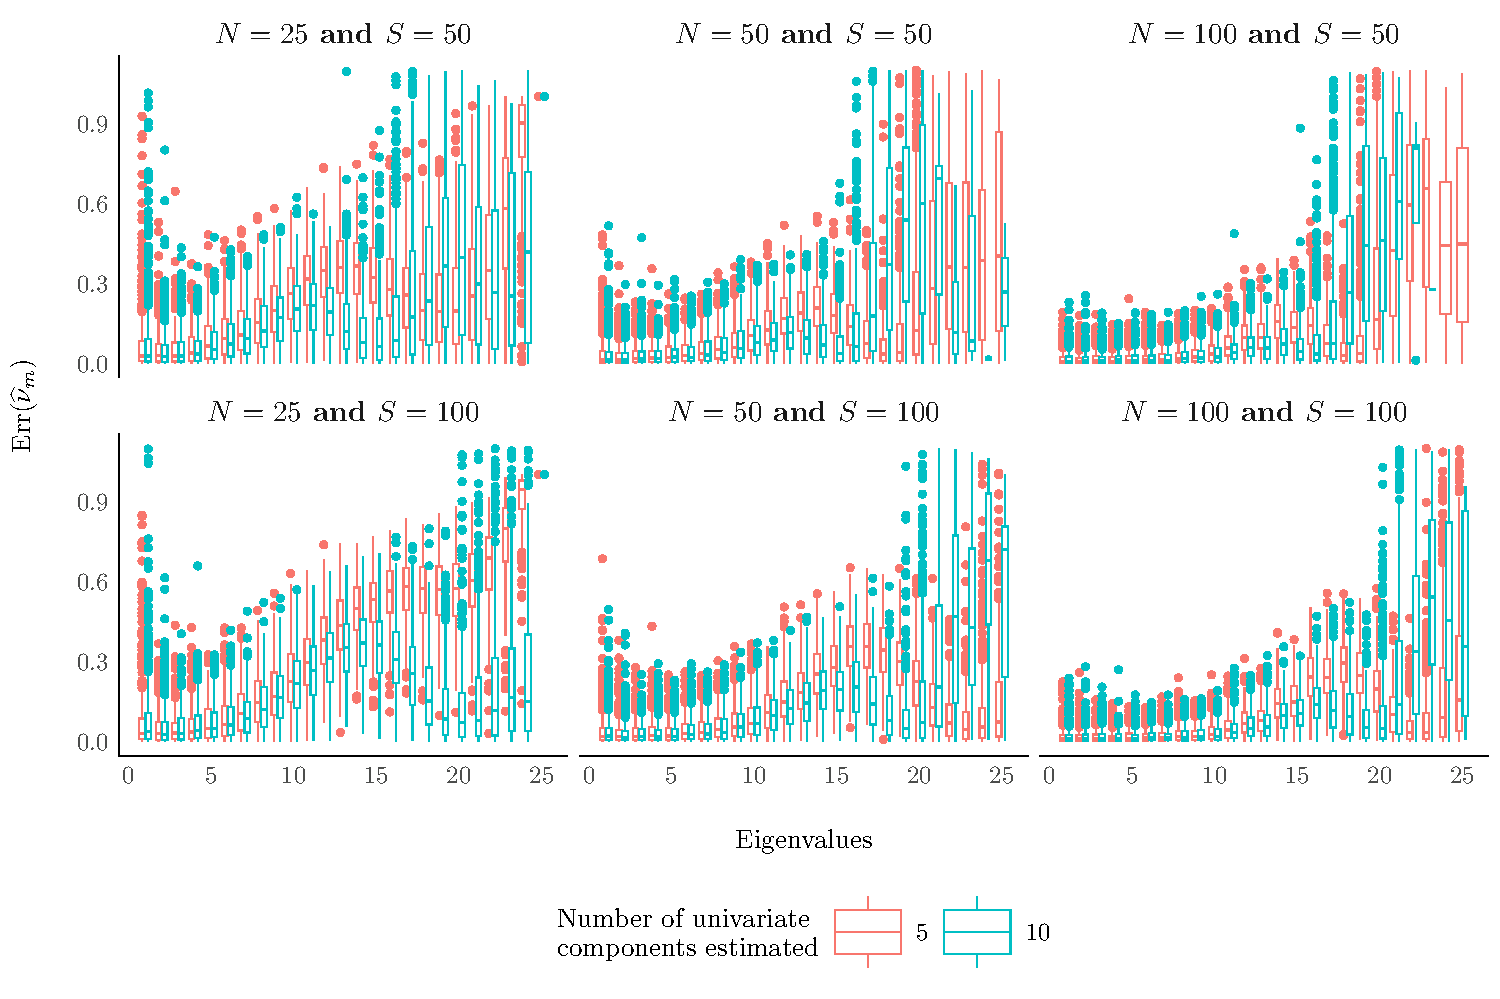
\includegraphics[width=0.94\textwidth]{ncomp.pdf}
    \caption{Boxplots of the estimation errors of the eigenvalues. We estimated $M_j = 5$ (red boxplots) and $M_j = 10$ (blue boxplots) univariate functional components for $j = 1, \dots, p$. The number of multivariate eigencomponents that are estimated is $25$. $N$ is the number of observations, $S$ is the number of sampling points per curve before the sparsification. We run $500$ simulations.}
    \label{fig:ncomp}
\end{figure}



\comments{The paragraph in the end of Page 2 and Page 3 requires a complete rewrite as it lacks the necessary rigor in its explanations and methodology.}

\reply{We have rewritten the paragraph to include more details on the methodology developed in \cite{happMultivariateFunctionalPrincipal2018} and which we comment on.}

\comments{The simulation study and application sections of the paper need to be significantly revised. The current writing provides very limited explanation, which makes it difficult for readers to fully understand the intuition behind the results, the significance of the findings, and how the method performs in practice. The authors should offer more detailed descriptions of the simulation settings including the rationale behind the chosen parameters and models. Moreover, the application section should clearly describe the dataset, the variables used, and how the results from the method apply to real-world scenarios. More emphasis should be placed on interpreting the application results and their implications which help readers understand the practical value of the proposed method.}

\reply{For the simulations, we added details on the results and their implications for practitioners.
For the application, we added a figure to visually present the dataset and included a new paragraph that provides a detailed interpretation of the eigencomponents. This paragraph highlights how the interpretation of the results differs between the two scenarios and explains their practical implications.}

\comments{The authors classify the number of simulations based on the size of the circles, which is very confusing. Please present the results using a clearer visualization method.}

\reply{We have replaced the plot with tables that present the results more clearly to enhances the readability and interpretability of the findings.}

\comments{The authors use B-spline bases for the Canadian weather dataset. I recommend that they also use a Fourier basis and compare the results. This can demonstrate the robustness of the method, as Fourier bases typically provide a better fit for weather data.}

\reply{Thank you for your suggestion to include a comparison using a Fourier basis. As our primary aim is to provide commentary on the estimation of the number of principal components utilising the methodology proposed in \cite{happMultivariateFunctionalPrincipal2018} and not finding the best representation of the data, we choose to not include the comparison into the main manuscript. We have included here the estimated eigenfunctions using $10$ Fourier basis functions for smoothing the Canadian weather dataset (see Fig.~\ref{fig:eigenfunctions_weather}). The estimated eigenfunctions obtained with the Fourier basis are consistent with those derived using the B-spline basis, demonstrating that the choice of basis does not affect the results in this case.}
\begin{figure}[!h]
     \centering
     \begin{subfigure}[b]{0.49\textwidth}
         \centering
         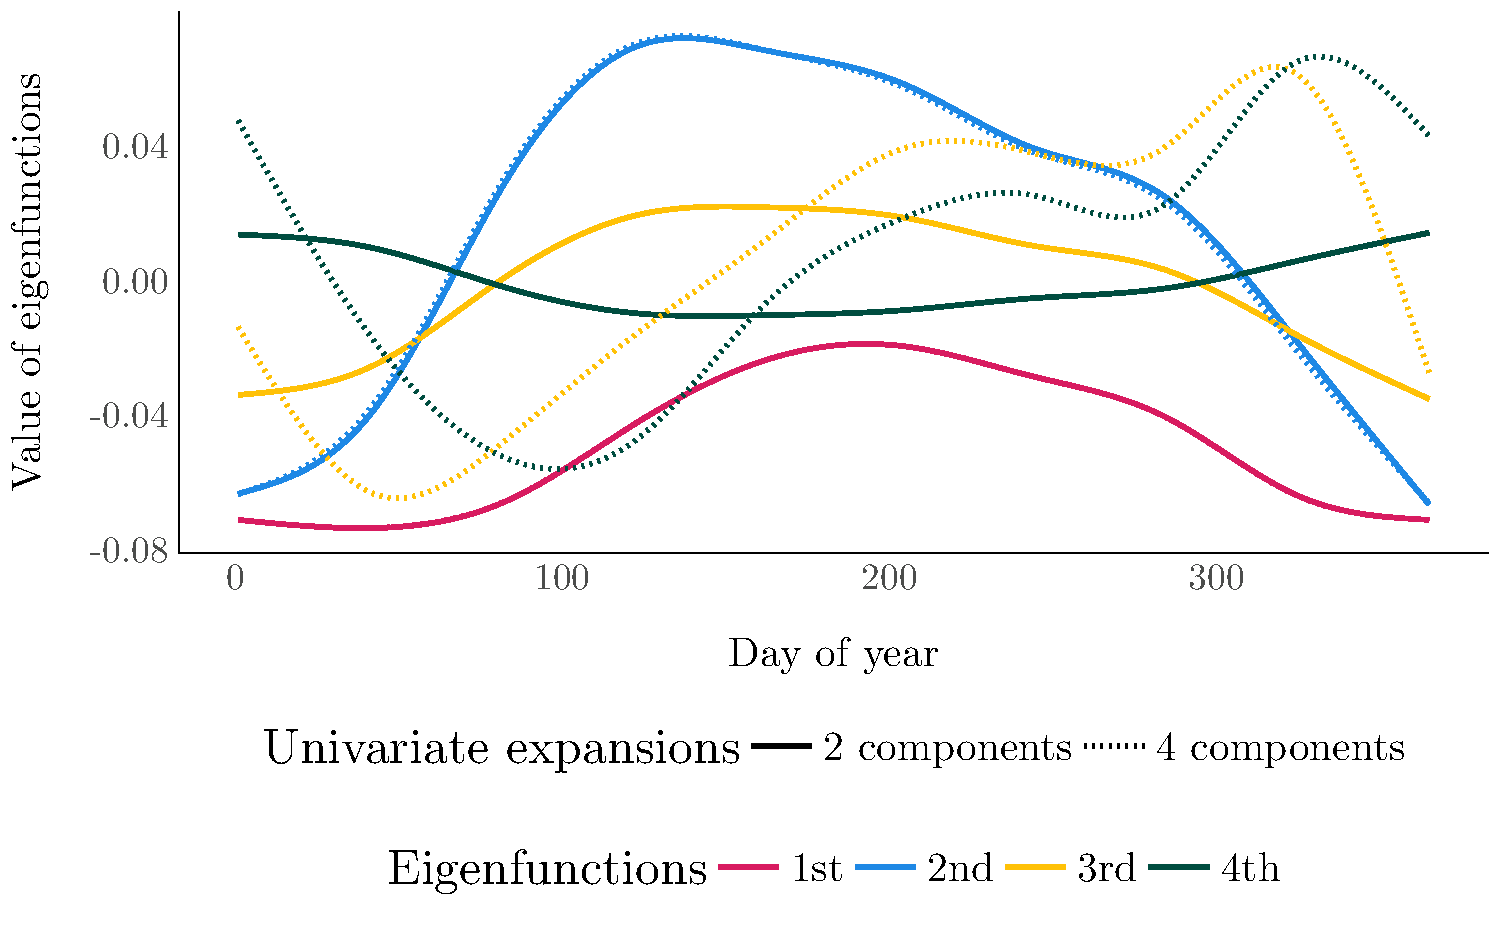
\includegraphics[width=1\textwidth]{temperature_eigen_fourier.pdf}
         \caption{Temperature (first component)}
         \label{fig:temperature}
     \end{subfigure}
     \hfill
     \begin{subfigure}[b]{0.49\textwidth}
         \centering
         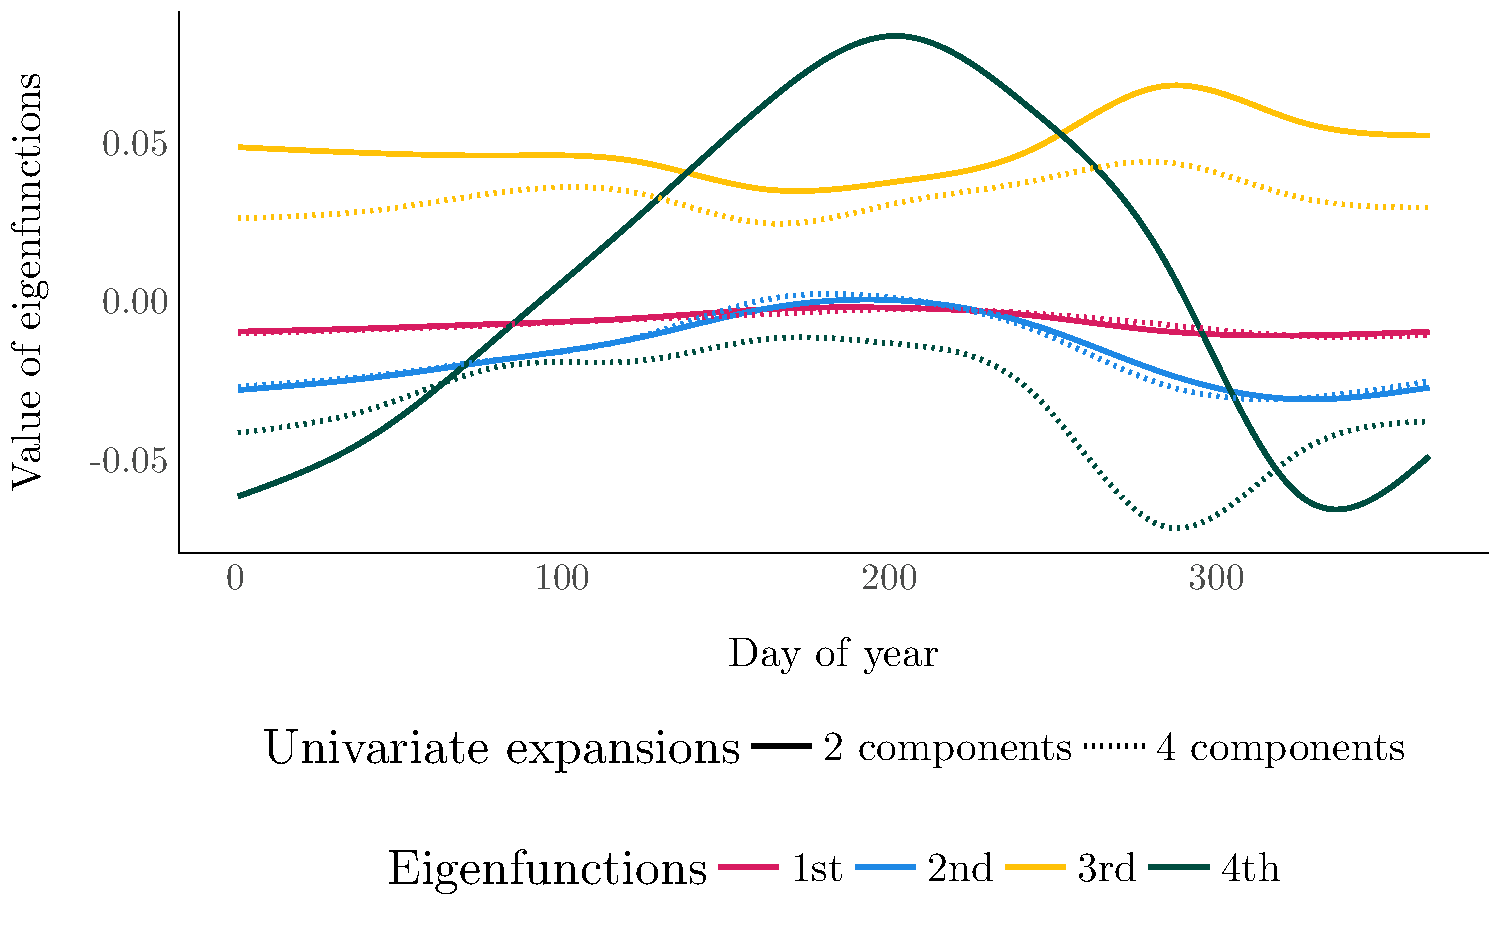
\includegraphics[width=1\textwidth]{precipitation_eigen_fourier.pdf}
         \caption{Precipitation (second component)}
         \label{fig:precipitation}
     \end{subfigure}
     \caption{Estimation of the first four eigenfunctions of the Canadian weather dataset using using two and four univariate components for the univariate expansions after Fourier basis smoothing.}
     \label{fig:eigenfunctions_weather}
\end{figure}



\comments{Figure 3 is missing a y-axis.}

\reply{We have updated Figure 3 to include the y-axis as ``Value of eigenfunctions''.}


\section{}


\comments{The manuscript needs English proofreading.}
\reply{The manuscript has been carefully revised by the three authors who are native English speakers.}


\comments{What is the limitation of the proposed approach?}
\reply{We would like to clarify that the primary aim of our manuscript is to ``provide commentary on the estimation of the number of principal components, utilising the methodology proposed in \cite{happMultivariateFunctionalPrincipal2018}''. We are not proposing a new methodology in this work but instead aim to critically evaluate and highlight the limitations of the approach introduced in \cite{happMultivariateFunctionalPrincipal2018}.}


%\bibliographystyle{plainnat}
\printbibliography
%\bibliography{biblio} 

\end{document} 